% !TEX root = ../main.tex
% 本文件由 build-tex.sh 从 21-DSP指南-第21章中译.md 生成，改内容请改 md 后重新生成

\chapter{滤波器比较}\label{ch-21}

选择，选择，还是选择！有这么多滤波器可选，怎么知道该用哪一个？本章是一场滤波器之间的正面对决：我们从各方选出冠军，让它们一决高下。第一场，数字滤波器(digital
filter)对阵模拟滤波器(analog filter)，看哪种技术更强。第二轮，加窗 sinc
滤波器(windowed-sinc filter)对阵切比雪夫滤波器(Chebyshev
filter)，争夺频域滤波器之王。最后一战，移动平均滤波器(moving average
filter)与单极点滤波器(single pole
filter)争夺时域冠军。废话少说，比赛开始！

\section{第一场：模拟滤波器 vs.~数字滤波器}

大多数数字信号都源自模拟电子电路。如果信号需要滤波，是在数字化之前用模拟滤波器好，还是数字化之后用数字滤波器好？我们让两位最强的选手过过招，来回答这个问题。

目标是实现一个 1 kHz
的低通滤波器。代表模拟一方出战的，是一个纹波(ripple)为 0.5
dB（6\%）的六极点切比雪夫滤波器。如第 3 章所述，它可以用 3
个运算放大器(op amp)、12 个电阻和 6 个电容搭出来。数字一方的角落里，加窗
sinc 滤波器已经热身完毕、准备开打。模拟信号以 10 kHz
的采样率数字化，于是截止频率在数字频率刻度上是 0.1。加窗 sinc 的长度选为
129 点，使它与模拟滤波器有相同的 90\% 到 10\%
滚降(roll-off)。公平起见。图 21-1
给出了这两个滤波器的频率响应和阶跃响应。

我们来逐招比较这两个滤波器。如 (a) 和 (b)
所示，模拟滤波器的通带(passband)有 6\%
的纹波，而数字滤波器完全平坦（误差在 0.02\%
以内）。模拟设计者可能会争辩说，纹波大小在设计时可以自己选；但这没抓住要点。模拟滤波器能达到的平坦度，受限于其电阻和电容的精度。即使设计成巴特沃斯响应(Butterworth
response，即 0\% 纹波)，这种复杂度的滤波器也会残留大约 1\%
的纹波。另一方面，数字滤波器的平坦度主要受舍入误差限制，比模拟滤波器平坦几百倍。数字滤波器得一分。

\begin{figure}[htbp]
\centering
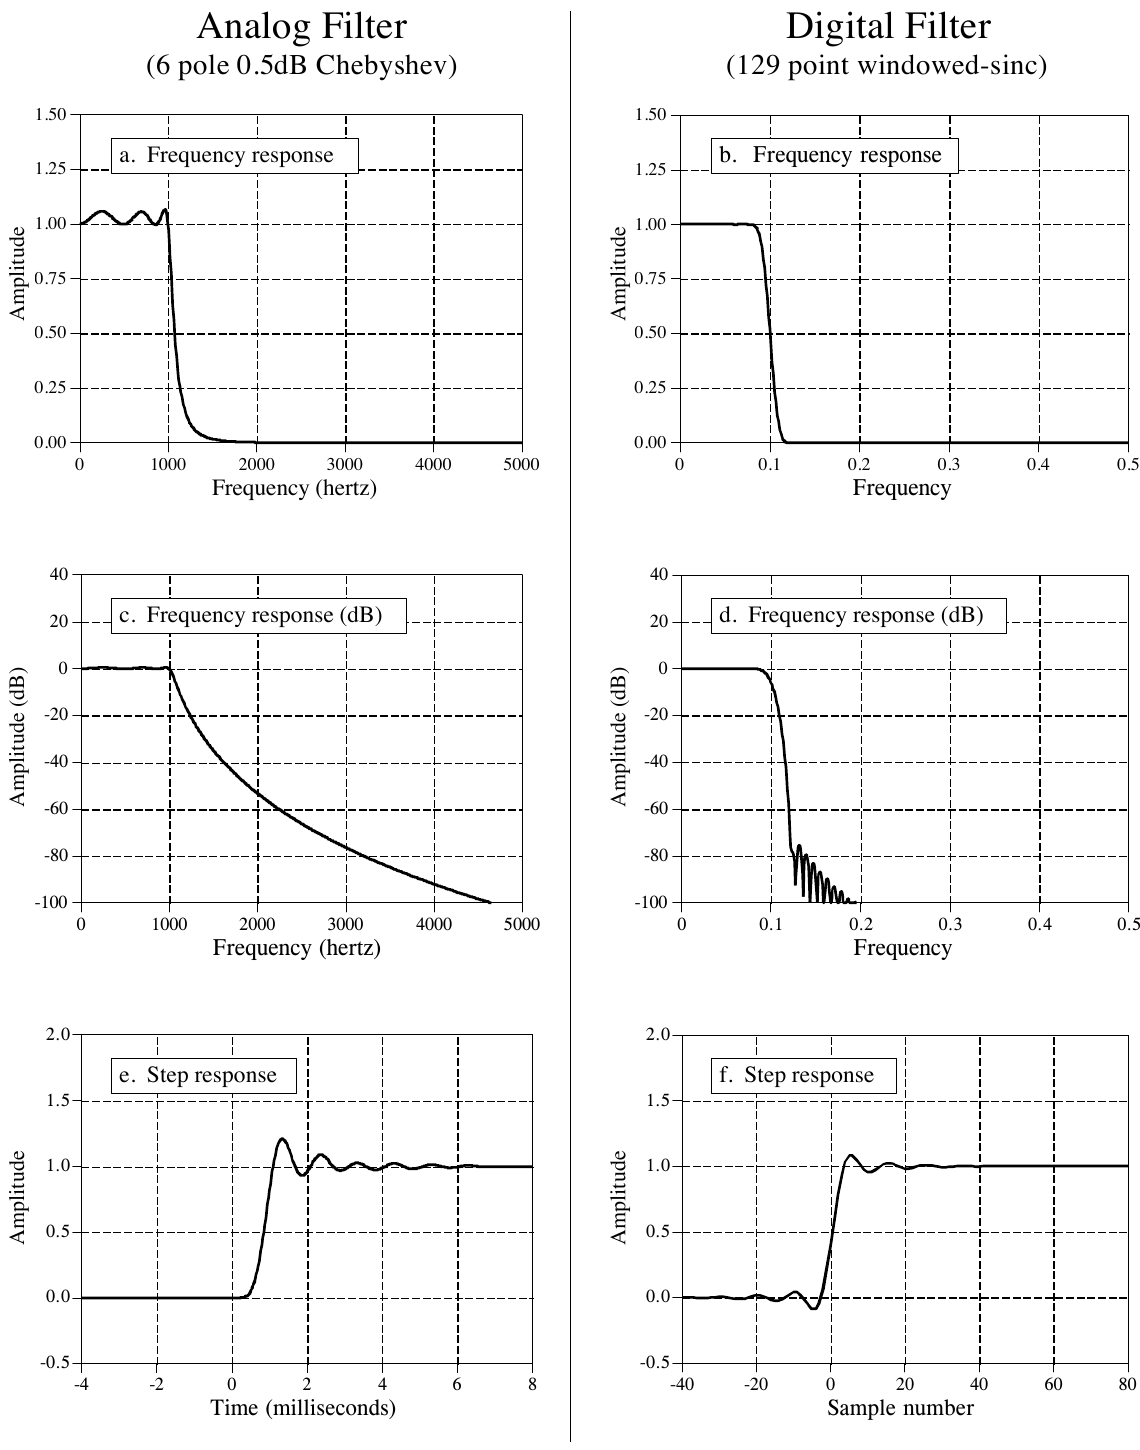
\includegraphics[width=0.950\linewidth,height=0.8\textheight,keepaspectratio]{assets/ch21/fig21-01.png}
\caption*{\textbf{图 21-1　模拟滤波器与数字滤波器的比较。}
数字滤波器在许多方面性能更好，例如：通带纹波，(a) 对
(b)；滚降和阻带衰减，(c) 对 (d)；阶跃响应的对称性，(e) 对
(f)。本例中数字滤波器的截止频率是 10 kHz 采样率的 0.1
倍，这样与模拟滤波器 1 kHz 的截止频率比较才公平。 （左栏 Analog Filter
(6 pole 0.5dB Chebyshev) = 模拟滤波器（六极点、0.5 dB 切比雪夫）；右栏
Digital Filter (129 point windowed-sinc) = 数字滤波器（129 点加窗
sinc）。a、b. Frequency response = 频率响应；c、d.~Frequency response
(dB) = 频率响应（dB）；e、f.~Step response = 阶跃响应。Amplitude =
幅度，Frequency (hertz) = 频率（赫兹），Frequency = 频率，Time
(milliseconds) = 时间（毫秒），Sample number = 采样序号。）}
\end{figure}

接下来看对数刻度下的频率响应，如 (c) 和 (d)
所示。在滚降和阻带衰减(stopband
attenuation)两方面，数字滤波器又一次明显获胜。即使给模拟电路再加几级来提高性能，它仍然没法和数字滤波器相比。例如，假设你需要把这两个参数提高
100 倍。对加窗 sinc
来说，简单改动就能做到；对模拟电路来说，这几乎不可能。数字滤波器再得两分。

两个滤波器的阶跃响应(step response)见 (e) 和
(f)。数字滤波器的阶跃响应在阶跃的下半段和上半段之间是对称的，也就是说它具有线性相位(linear
phase)。模拟滤波器的阶跃响应不对称，也就是说它具有非线性相位(nonlinear
phase)。数字滤波器再得一分。最后，模拟滤波器在阶跃的一侧过冲(overshoot)约
20\%；数字滤波器过冲约
10\%，但阶跃两侧都有。既然两者都不好，这一项不给分。

尽管被打得这么惨，仍然有许多应用应该、甚至必须用模拟滤波器。这和滤波器本身的性能（即输入什么、输出什么）无关，而在于模拟电路相对数字技术的一般优势。第一个优势是速度：数字慢，模拟快。例如，个人计算机用
FFT 卷积，每秒只能处理大约 10,000
个采样。而即使是简单的运算放大器，也能工作在 100 kHz 到 1
MHz，比数字系统快 10 到 100 倍！

模拟相对数字的第二个固有优势是动态范围(dynamic
range)。它有两种。幅度动态范围(amplitude dynamic
range)是系统能通过的最大信号与系统固有噪声之比。例如，一个 12 位 ADC
的饱和电平是 4095，均方根量化噪声是 0.29 个数字量，动态范围约为
14000。相比之下，一个普通运算放大器的饱和电压约 20 伏，内部噪声约 2
微伏，动态范围约为一千万。和前面一样，一个简单的运算放大器就把数字系统打得落花流水。

另一种是频率动态范围(frequency dynamic range)。例如，设计一个能同时处理
0.01 Hz 到 100
kHz（七个十倍程）频率的运放电路很容易。用数字系统去做，计算机就会被数据淹没。比如以
200 kHz 采样，要捕获 0.01 Hz 的一个完整周期需要 2000
万个点。你可能注意到了，数字滤波器的频率响应几乎总是画在线性频率刻度上，而模拟滤波器通常用对数频率显示。这是因为数字滤波器需要线性刻度来展示它们出色的滤波性能，而模拟滤波器需要对数刻度来展示它们巨大的动态范围。

\section{第二场：加窗 sinc vs.~切比雪夫}

加窗 sinc
滤波器和切比雪夫滤波器都是为了把一个频带与另一个频带分开而设计的。加窗
sinc 是用卷积实现的 FIR 滤波器，而切比雪夫是用递归实现的 IIR
滤波器。在频域里，哪个是最好的数字滤波器？我们让它们打一场。

递归滤波器一方的选手是一个纹波
0.5\%、六极点的切比雪夫低通滤波器。要做到公平比较并不简单，因为切比雪夫的频率响应会随截止频率而变。我们用
0.2 的截止频率，并把加窗 sinc 的滤波器核选为 51
点。这样两个滤波器就有相同的 90\% 到 10\% 滚降，如图 21-2(a) 所示。

推推搡搡开始了。递归滤波器的通带有 0.5\% 的纹波，而加窗 sinc
是平坦的。不过，如果需要，我们很容易把递归滤波器的纹波设成
0\%。不给分。图 21-2b 显示加窗 sinc 的阻带衰减比切比雪夫好得多。加窗
sinc 得一分。

\begin{figure}[htbp]
\centering
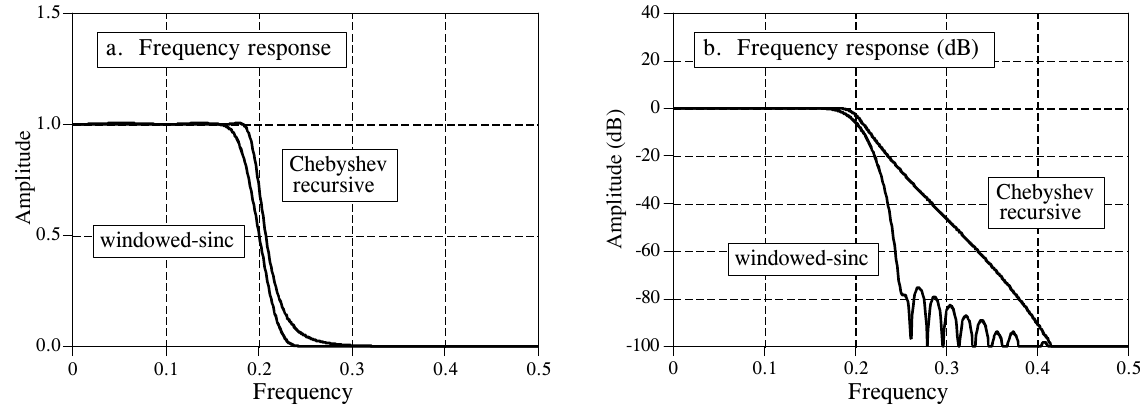
\includegraphics[width=0.950\linewidth,height=0.8\textheight,keepaspectratio]{assets/ch21/fig21-02.png}
\caption*{\textbf{图 21-2　加窗 sinc 与切比雪夫的频率响应。} 图中是 51 点加窗 sinc
滤波器和六极点、0.5\% 纹波切比雪夫递归滤波器的频率响应。加窗 sinc
的阻带衰减更好，但在性能要求中等的应用中两者都能用。两个滤波器的截止频率都是
0.2；对加窗 sinc 是在幅度 0.5 处测量，对递归滤波器是在 0.707 处测量。
（a. Frequency response = 频率响应；b. Frequency response (dB) =
频率响应（dB）。windowed-sinc = 加窗 sinc，Chebyshev recursive =
切比雪夫递归。Amplitude = 幅度，Frequency = 频率。）}
\end{figure}

图 21-3
给出了两个滤波器的阶跃响应。两者都很差，这对频域滤波器来说是意料之中的。递归滤波器是非线性相位，但可以用双向滤波(bidirectional
filtering)来校正。既然两个滤波器在这一项上都这么难看，就算平局。

\begin{figure}[htbp]
\centering
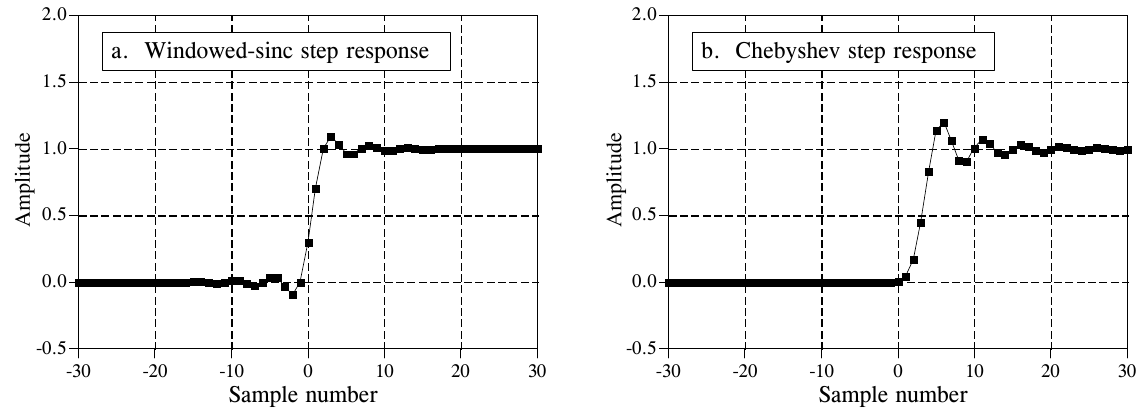
\includegraphics[width=0.950\linewidth,height=0.8\textheight,keepaspectratio]{assets/ch21/fig21-03.png}
\caption*{\textbf{图 21-3　加窗 sinc 与切比雪夫的阶跃响应。} 图中是 51 点加窗 sinc
滤波器和六极点、0.5\%
纹波切比雪夫递归滤波器的阶跃响应，两者的截止频率都是 0.2。加窗 sinc
的阶跃响应略好一些，因为它的过冲更小，而且是零相位(zero phase)。 （a.
Windowed-sinc step response = 加窗 sinc 阶跃响应；b. Chebyshev step
response = 切比雪夫阶跃响应。Amplitude = 幅度，Sample number =
采样序号。原书图注把 Windowed-sinc 印成了 Windowed--sinc。）}
\end{figure}

到目前为止，这两个滤波器差别不大；需要中等性能时，用哪个都行。真正的重拳出在两个关键问题上：最高性能和速度。加窗
sinc
是大力士，而切比雪夫灵活敏捷。假设你遇到一个非常棘手的频率分离问题，比如要从一条
60 赫兹、120 伏的电源线上，分离出骑在上面的一个 61 赫兹、100
毫伏的信号。图 21-4
展示了需要最高性能时这两个滤波器的对比。递归滤波器是纹波 0.5\%
的六极点切比雪夫，这是单精度下截止频率 0.05 时能用的最多极点数。加窗
sinc 使用 1001 点的滤波器核，它由一个 501 点加窗 sinc
滤波器核与自身卷积而成。如第 16 章所示，这样能得到更大的阻带衰减。

\begin{figure}[htbp]
\centering
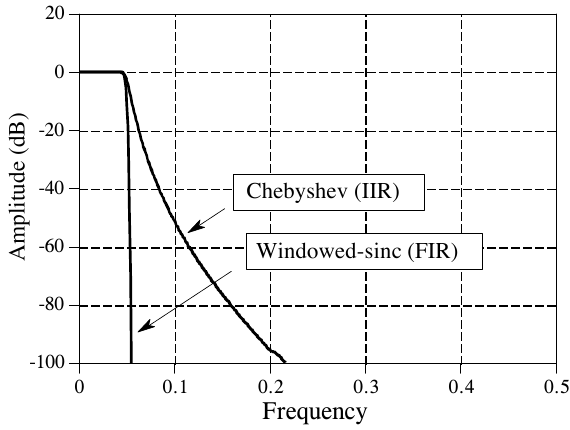
\includegraphics[width=0.475\linewidth,height=0.8\textheight,keepaspectratio]{assets/ch21/fig21-04.png}
\caption*{\textbf{图 21-4　FIR 与 IIR 滤波器的最高性能。} 加窗 sinc
的频率响应几乎可以做成任何需要的形状，而切比雪夫递归滤波器则非常受限。这张图比较了六极点切比雪夫递归滤波器与
1001 点加窗 sinc 滤波器的频率响应。 （Chebyshev (IIR) =
切比雪夫（IIR），Windowed-sinc (FIR) = 加窗 sinc（FIR）。Amplitude (dB)
= 幅度（dB），Frequency =
频率。原书说明排在图的左侧，裁图时已去掉，译文见上。）}
\end{figure}

需要最高性能时，这两个滤波器比起来怎样？加窗 sinc
完胜切比雪夫！即使改进递归滤波器（更多极点、多级实现、双精度等等），它也仍然比不上
FIR 的性能。想到加窗 sinc
才刚刚开始发力，这就更令人印象深刻了。递归滤波器能提供的最高性能有很强的限制；相反，加窗
sinc
可以被推到不可思议的水平。当然，前提是你愿意等结果。这就引出了第二个关键问题：速度。

比较这两个滤波器的速度，就像让法拉利和卡丁车赛跑。图 21-5 显示了加窗
sinc
相比六极点递归滤波器要多花多少执行时间。由于递归滤波器在低频和高频处滚降更快，加窗
sinc
的核必须做得更长才能匹配其性能（也就是为了保持比较的公平）。这就是加窗
sinc 在频率 0 和 0.5 附近执行时间增加的原因。重点是：可以预期 FIR
滤波器比性能相当的 IIR 滤波器慢大约一个数量级（卡丁车：15
英里/小时，法拉利：150 英里/小时）。

\begin{figure}[htbp]
\centering
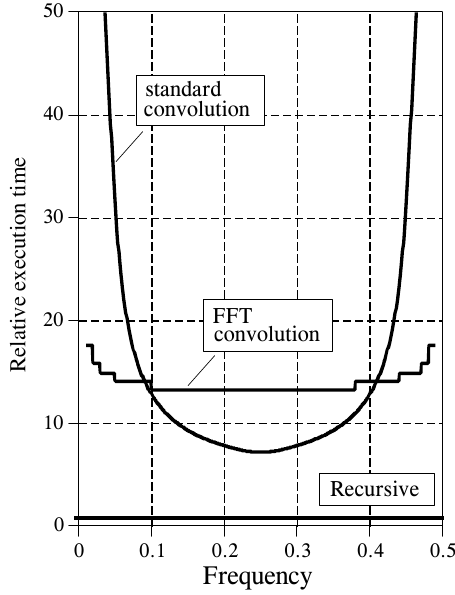
\includegraphics[width=0.379\linewidth,height=0.8\textheight,keepaspectratio]{assets/ch21/fig21-05.png}
\caption*{\textbf{图 21-5　FIR 与 IIR 执行速度的比较。} 这些曲线给出了加窗 sinc
滤波器相对于等效的六极点切比雪夫递归滤波器的执行时间。FIR
滤波器分别用标准卷积和 FFT 卷积两种算法实现，各画了一条曲线。加窗 sinc
的执行时间在低频和高频处上升，因为在这些频率上递归滤波器性能更强，滤波器核必须加长才能跟上。一般来说，IIR
滤波器比性能相当的 FIR 滤波器快一个数量级。 （standard convolution =
标准卷积，FFT convolution = FFT 卷积，Recursive = 递归。Relative
execution time = 相对执行时间，Frequency =
频率。原书说明排在图的左侧，裁图时已去掉，译文见上。）}
\end{figure}

\section{第三场：移动平均 vs.~单极点}

第三场比赛是时域滤波器之战。第一位选手是一个 9
点移动平均滤波器。今天它的对手是一个使用双向技术的单极点递归滤波器。为了得到可比的频率响应，单极点滤波器使用的逐采样衰减系数为
\(x = 0.70\)。战斗从图 21-6
开始，图中给出了两个滤波器各自的频率响应。两者都不怎么样，不过当然，频率分离本来就不是这些滤波器的用途。双方都不得分。

\begin{figure}[htbp]
\centering
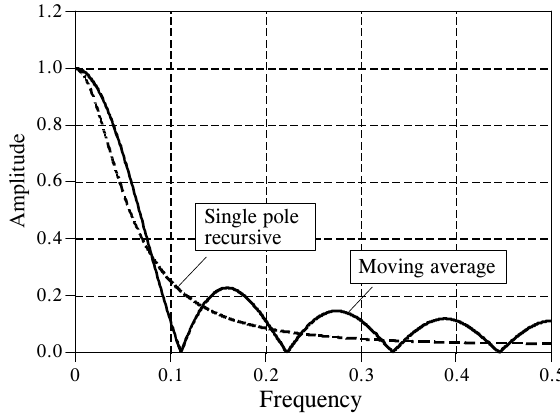
\includegraphics[width=0.467\linewidth,height=0.8\textheight,keepaspectratio]{assets/ch21/fig21-06.png}
\caption*{\textbf{图 21-6　移动平均与单极点滤波器的频率响应。}
这两个滤波器的频率响应都很差，这对时域滤波器来说是意料之中的。 （Single
pole recursive = 单极点递归（虚线），Moving average =
移动平均（实线）。Amplitude = 幅度，Frequency =
频率。原书说明排在图的左侧，裁图时已去掉，译文见上。）}
\end{figure}

图 21-7 给出了两个滤波器的阶跃响应。在 (a)
中，移动平均的阶跃响应是一条直线，这是从一个电平变到另一个电平最快的方式。在
(b) 中，递归滤波器的阶跃响应更平滑，在某些应用中可能更好。双方各得一分。

\begin{figure}[htbp]
\centering
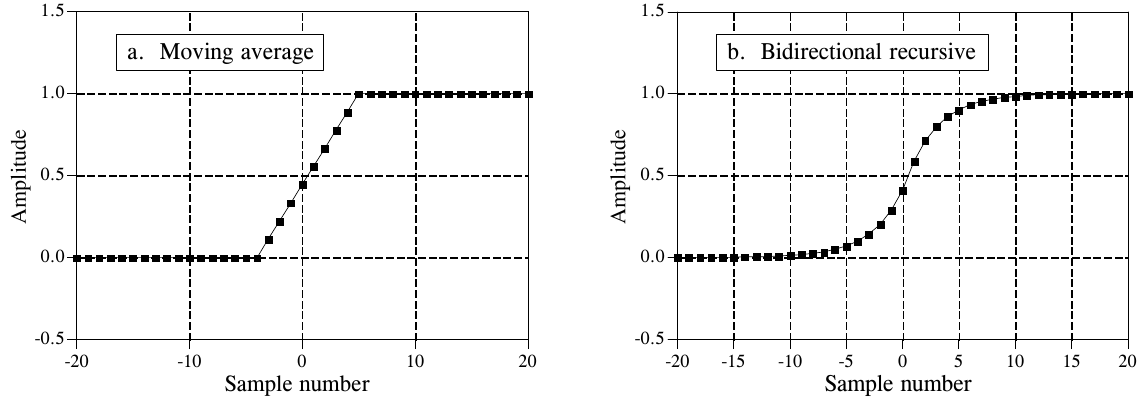
\includegraphics[width=0.950\linewidth,height=0.8\textheight,keepaspectratio]{assets/ch21/fig21-07.png}
\caption*{\textbf{图 21-7　移动平均与双向单极点滤波器的阶跃响应。}
移动平均的阶跃响应在更少的采样内完成，而单极点滤波器的阶跃响应更平滑。
（a. Moving average = 移动平均；b. Bidirectional recursive =
双向递归。Amplitude = 幅度，Sample number = 采样序号。）}
\end{figure}

这两个滤波器在性能上势均力敌，两者之间的选择往往取决于个人偏好。不过，有两种情况下其中一个略占上风。它们取决于开发时间与执行时间之间的权衡。第一种情况，你想缩短开发时间，愿意接受较慢的滤波器。例如，你可能只是一次性地需要过滤几千个点。整个程序几秒钟就跑完，花时间优化算法毫无意义。几乎肯定会用浮点数。可选的是用卷积实现的移动平均滤波器，或者单极点递归滤波器。这里的赢家是递归滤波器：它编写和修改起来稍微容易一点，而且执行快得多。

第二种情况正好相反：你的滤波器必须尽可能快，你也愿意多花开发时间来做到这一点。例如，这个滤波器可能是某个商业产品的一部分，可能要运行几百万次。为了获得最高速度，你可能会用整数。可选的滤波器是用递归实现的移动平均滤波器，或者用查找表(look-up
table)或整数运算实现的单极点递归滤波器。赢家是移动平均滤波器：它执行更快，也不会受到整数运算在开发和执行上的那些问题影响。
